\chapter{System morphology}
In this section we describe how the to specify the morphology of the system. We will use DCV2T as an example.

\section{Single molecule}

\begin{wrapfigure}{ht}{0.6\linewidth}
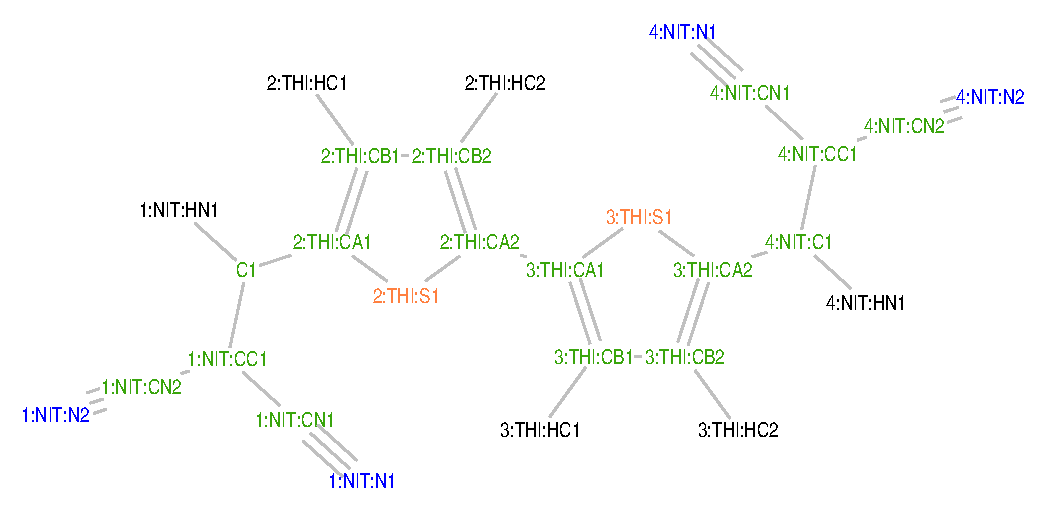
\includegraphics[width=\linewidth]{./fig/chemical_structure/dcv2t_atom_types}
\caption{\small Atom types of DCV2T. The molecule has two types of building blocks (residues), thiophene (THI) and dicyanovinyl (NIT). }
\label{fig:dcv2t_at}
\end{wrapfigure}

%\clearpage
The structure of DCV2T, together with atom type definitions, is shown in fig.~\ref{fig:dcv2t_at}. DCV2T is a typical donor-acceptor-type molecule, with two electron-donating thiophene and two electron-withdrawing dicyanovinyl groups. The pdb file which contains residue types, residue numbering, atom names, atom types, and atom coordinates is shown below. There are two residue types, THI, and NIT, for the thiophene and dicyanovinyl groups, respectively. In its ground state the molecule is practically planar. 

\VerbatimInput[%
frame=lines,
framesep=4mm,
label=\fbox{pdb file of DCV2T}, 
framerule=0.5mm,
rulecolor=\color{red},
baselinestretch=1,
fontsize=\footnotesize%,
%numbers=left
]%
{./fig/chemical_structure/dcv2t.pdb}


\section{Large-scale morphology}